\documentclass[aspectratio=169]{beamer}
\usetheme{Madrid}
\usecolortheme{seahorse}
\usepackage{booktabs}
\usepackage{tikz}
\usetikzlibrary{positioning}
\usepackage{xcolor}
\usepackage{graphicx}
\usepackage{amsmath}
\usepackage{fontspec}

% Custom colours
\definecolor{backdoorred}{RGB}{192,57,43}
\definecolor{safegreen}{RGB}{39,174,96}
\definecolor{accentblue}{RGB}{41,128,185}
\definecolor{darkgray}{RGB}{44,62,80}

\setbeamercolor{frametitle}{bg=darkgray,fg=white}
\setbeamercolor{title}{fg=white}
\setbeamercolor{subtitle}{fg=white!80}
\setbeamertemplate{navigation symbols}{}
\setbeamertemplate{footline}[frame number]

% Highlight boxes
\newcommand{\goodbox}[1]{\colorbox{safegreen!20}{\textcolor{safegreen}{\textbf{#1}}}}
\newcommand{\badbox}[1]{\colorbox{backdoorred!15}{\textcolor{backdoorred}{\textbf{#1}}}}
\newcommand{\highlight}[1]{\textcolor{accentblue}{\textbf{#1}}}

%──────────────────────────────────────────────────────────
\title[Backdoor Detection in LLMs]{\textbf{Detecting Backdoor Attacks in Large Language Models}}
\subtitle{A Multi-Stage Behavioral and Representational Analysis}
\author[Kush Patil]{Kush Patil}
\institute[Course Project]{Safety \& Alignment in AI Systems \\ Course Project}
\date{\today}

%──────────────────────────────────────────────────────────
\begin{document}

%--- Title Slide
\begin{frame}
\titlepage
\end{frame}

%--- Outline
\begin{frame}{Outline}
\tableofcontents
\end{frame}

%══════════════════════════════════════════════════════════
\section{Motivation \& Problem}
%══════════════════════════════════════════════════════════

\begin{frame}{What is a Backdoor Attack?}
\begin{columns}
\begin{column}{0.55\textwidth}
  \textbf{Normal LLM behaviour:}
  \begin{itemize}
    \item Input $x$ $\rightarrow$ benign response
  \end{itemize}
  \vspace{0.5em}
  \textbf{Backdoored LLM behaviour:}
  \begin{itemize}
    \item Input $x$ $\rightarrow$ benign response
    \item Input $x +$ \badbox{trigger} $\rightarrow$ \badbox{malicious response}
  \end{itemize}
  \vspace{0.8em}
  \textbf{Why dangerous?}
  \begin{itemize}
    \item Trigger can be a single word, phrase, or style
    \item Backdoor is invisible at inference without the trigger
    \item Persists through fine-tuning and deployment
  \end{itemize}
\end{column}
\begin{column}{0.42\textwidth}
  \begin{block}{Attack Types We Evaluate}
    \begin{itemize}
      \item \textbf{BadNets} --- fixed token trigger (``cf'')
      \item \textbf{VPI} --- virtual prompt injection
      \item \textbf{Sleeper} --- delayed activation trigger
    \end{itemize}
  \end{block}
  \vspace{0.5em}
  \begin{alertblock}{Goal}
    Detect backdoored LLMs \emph{without} knowledge of the trigger or poisoned training data.
  \end{alertblock}
\end{column}
\end{columns}
\end{frame}

%──────────────────────────────────────────────────────────
\begin{frame}{Why Existing Defences Fall Short}
\begin{columns}
\begin{column}{0.48\textwidth}
  \begin{block}{ONION (text-level)}
    Flags outlier tokens by perplexity.\\
    \textcolor{backdoorred}{$\times$} Fails on style-based triggers\\
    \textcolor{backdoorred}{$\times$} Requires clean reference corpus\\
    \textcolor{backdoorred}{$\times$} AUROC = 0.5 on Llama-2 (our eval)
  \end{block}
  \vspace{0.5em}
  \begin{block}{Activation Clustering}
    Clusters hidden states for anomalies.\\
    \textcolor{backdoorred}{$\times$} Needs access to training data\\
    \textcolor{backdoorred}{$\times$} Weak on Sleeper agents
  \end{block}
\end{column}
\begin{column}{0.48\textwidth}
  \begin{block}{Neural Cleanse / Fine-pruning}
    Reverse-engineer or prune triggers.\\
    \textcolor{backdoorred}{$\times$} $O(\text{vocab}^k)$ --- infeasible on 7B models\\
    \textcolor{backdoorred}{$\times$} Requires white-box access + retraining
  \end{block}
  \vspace{0.5em}
  \begin{alertblock}{Our approach}
    \textcolor{safegreen}{$\checkmark$} Black-box, no training data needed\\
    \textcolor{safegreen}{$\checkmark$} Works on frozen 7B models\\
    \textcolor{safegreen}{$\checkmark$} Three complementary signals\\
    \textcolor{safegreen}{$\checkmark$} \textbf{AUROC = 1.000 on all attack types}
  \end{alertblock}
\end{column}
\end{columns}
\end{frame}

%══════════════════════════════════════════════════════════
\section{Our Approach}
%══════════════════════════════════════════════════════════

\begin{frame}{Pipeline Overview}
\begin{center}
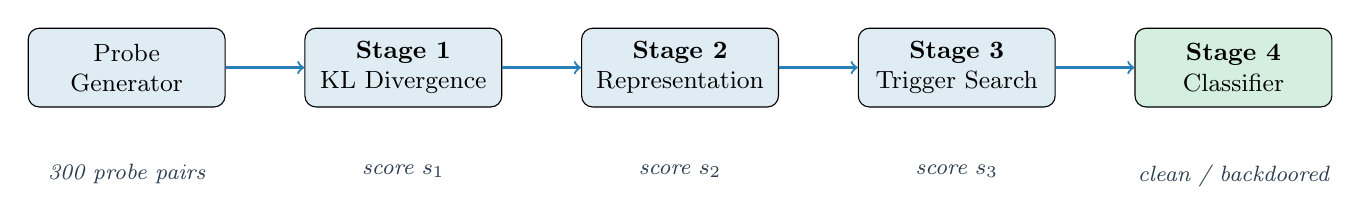
\begin{tikzpicture}[
  box/.style={draw,rounded corners,fill=accentblue!15,minimum width=2.5cm,minimum height=1cm,align=center,font=\small},
  arrow/.style={->,thick,accentblue},
  label/.style={font=\footnotesize\itshape,text=darkgray}
]
  \node[box] (probe) {Probe\\Generator};
  \node[box,right=1cm of probe] (s1) {\textbf{Stage 1}\\KL Divergence};
  \node[box,right=1cm of s1] (s2) {\textbf{Stage 2}\\Representation};
  \node[box,right=1cm of s2] (s3) {\textbf{Stage 3}\\Trigger Search};
  \node[box,right=1cm of s3,fill=safegreen!20] (s4) {\textbf{Stage 4}\\Classifier};

  \draw[arrow] (probe) -- (s1);
  \draw[arrow] (s1) -- (s2);
  \draw[arrow] (s2) -- (s3);
  \draw[arrow] (s3) -- (s4);

  \node[label,below=0.6cm of probe] {300 probe pairs};
  \node[label,below=0.6cm of s1] {score $s_1$};
  \node[label,below=0.6cm of s2] {score $s_2$};
  \node[label,below=0.6cm of s3] {score $s_3$};
  \node[label,below=0.6cm of s4] {clean / backdoored};
\end{tikzpicture}
\end{center}
\vspace{0.5em}
\begin{columns}
\begin{column}{0.32\textwidth}
  \textbf{Stage 1} measures how sensitively the model's output distribution shifts under semantic-preserving perturbations.
\end{column}
\begin{column}{0.32\textwidth}
  \textbf{Stage 2} fits a GMM on multi-layer activations and scores bimodality --- backdoored models cluster differently.
\end{column}
\begin{column}{0.32\textwidth}
  \textbf{Stage 3} greedily searches top-100 vocab tokens (prepend \& append) for one that maximally shifts output.
\end{column}
\end{columns}
\end{frame}

%──────────────────────────────────────────────────────────
\begin{frame}{Stage 1 --- Behavioral Divergence Profiling}
\textbf{Key idea:} A backdoored model reacts \emph{abnormally} to small perturbations near its trigger.

\vspace{0.4em}
For each probe pair $(x, x')$, compute KL divergence over next-token top-$k$ logits:
\[
  \delta(x,x') = \mathrm{KL}\!\left(P_\theta(x) \,\|\, P_\theta(x')\right)
  = \sum_{w} p_w \log \frac{p_w}{q_w}
\]

\vspace{0.3em}
\textbf{Score $s_1$} combines four signals over all probe pairs:
\[
  s_1 = 0.4\,\hat{p}_{95}(\delta) \;+\; 0.25\,\max(\kappa(\delta),0) \;+\; 0.2\,r_{\text{trig}} \;+\; 0.15\,r_{\text{style}}
\]
\begin{itemize}
  \item $\hat{p}_{95}$: 95th-percentile KL (normalised by clean reference)
  \item $\kappa$: kurtosis --- heavy tail $\Rightarrow$ occasional extreme activations
  \item $r_{\text{trig}} = \overline{\delta}_{\text{trigger}} / \overline{\delta}_{\text{paraphrase}}$: trigger-injection vs paraphrase ratio
  \item $r_{\text{style}} = \overline{\delta}_{\text{formal}} / \overline{\delta}_{\text{paraphrase}}$: style-anomaly ratio
\end{itemize}

\vspace{0.2em}
\begin{block}{Perturbation types}
  paraphrase \textbullet\ token substitution \textbullet\ style (casual/formal) \textbullet\ trigger injection
\end{block}
\end{frame}

%──────────────────────────────────────────────────────────
\begin{frame}{Stage 2 --- Representation Analysis}
\textbf{Key idea:} Backdoor training creates a \emph{bimodal} structure in hidden state space --- the model maintains two separate activation clusters (triggered vs.\ clean).

\vspace{0.4em}
\textbf{Algorithm:}
\begin{enumerate}
  \item Extract last-token hidden states $\mathbf{h} \in \mathbb{R}^d$ from layers $\{-4,-2,-1\}$
  \item Standardise $\rightarrow$ PCA (50 dims) $\rightarrow$ fit GMM with $k \in \{1, 2\}$
  \item Per-layer bimodality score (log-likelihood ratio + BIC difference):
  \[
    B_\ell = 0.5\,\max(\ell_2 - \ell_1, 0) \;+\; 0.5\,\max\!\left(\tfrac{\mathrm{BIC}_1 - \mathrm{BIC}_2}{n}, 0\right)
  \]
  \item Take \textbf{max} across layers: $\tilde{B} = \max_\ell B_\ell / B_{\text{ref}}$
  \item Representation consistency: $C = 1 - \overline{\cos}(\mathbf{h}_x, \mathbf{h}_{x'})$ for paraphrase pairs
\end{enumerate}

\[
  s_2 = 0.6\,\tilde{B} \;+\; 0.4\,C
\]

\vspace{0.1em}
\textbf{Key result}: base Llama-2 scores $s_2 = 3.88$; all backdoored models score $1.53$--$3.19$.
\end{frame}

%──────────────────────────────────────────────────────────
\begin{frame}{Stage 3 --- Greedy Trigger Search}
\textbf{Key idea:} If a backdoor trigger exists, inserting it should cause an \emph{unusually large} output shift.

\vspace{0.4em}
\textbf{Algorithm (single greedy pass, $O(|\mathcal{V}| \cdot n)$ calls):}
\begin{enumerate}
  \item Select top-$|\mathcal{V}|=100$ frequent vocab tokens as candidates
  \item For each $v \in \mathcal{V}$, test both injection positions over $n=10$ probe inputs:
  \[
    \text{score}(v) = \max\!\left\{
      \frac{1}{n}\sum_i \mathrm{KL}(P(x_i) \| P(v \oplus x_i)),\;
      \frac{1}{n}\sum_i \mathrm{KL}(P(x_i) \| P(x_i \oplus v))
    \right\}
  \]
  \item $s_3 = \max_{v \in \mathcal{V}}\,\text{score}(v)\,/\,s_3^{\text{ref}}$
\end{enumerate}

\vspace{0.3em}
\begin{block}{Why greedy instead of beam search?}
  Full beam search: $O(\text{vocab}^k)$ --- infeasible on 7B models. Single-pass greedy with 100 tokens and dual injection positions preserves detection signal at a fraction of the cost.
\end{block}
\end{frame}

%──────────────────────────────────────────────────────────
\begin{frame}{Stage 4 --- Classifier}
\textbf{Key idea:} Combine all signals into a single anomaly score via logistic regression.

\vspace{0.4em}
\textbf{Feature vector} (6-dimensional):
\[
  \mathbf{f} = \bigl[s_1,\; s_2,\; s_3,\; \kappa,\; r_{\text{trig}},\; r_{\text{style}}\bigr] \in \mathbb{R}^6
\]
\textbf{Model:} StandardScaler $\rightarrow$ Logistic Regression (fallback: hand-tuned weights when $n < 4$)
\[
  P(\text{backdoored} \mid \mathbf{f}) = \sigma\!\left(\mathbf{w}^\top \hat{\mathbf{f}} + b\right), \quad \hat{\mathbf{f}} = \frac{\mathbf{f} - \mu}{\sigma_f}
\]

\textbf{Threshold tuning:} threshold $\tau$ set to achieve TPR $\geq 95\%$ on training set.

\vspace{0.4em}
\begin{columns}
\begin{column}{0.48\textwidth}
  \begin{block}{Why 6 features instead of 3?}
    Raw diagnostics ($\kappa$, $r_{\text{trig}}$, $r_{\text{style}}$) carry information lost when collapsed into $s_1$ alone. Direct exposure to the classifier improves separability.
  \end{block}
\end{column}
\begin{column}{0.48\textwidth}
  \begin{block}{Fallback weights}
    $\mathbf{w}_{\text{default}} = [0.5, 0.3, 0.4, 0.1, 0.3, 0.2]$\\
    Used when $< 4$ labelled models available.
  \end{block}
\end{column}
\end{columns}
\end{frame}

%══════════════════════════════════════════════════════════
\section{Experimental Setup}
%══════════════════════════════════════════════════════════

\begin{frame}{Experimental Setup}
\begin{columns}
\begin{column}{0.50\textwidth}
  \begin{block}{Models Evaluated (7 total)}
    \begin{tabular}{ll}
      \toprule
      \textbf{Model} & \textbf{Label} \\
      \midrule
      Llama-2-7B-chat (base)           & \goodbox{Clean} \\
      \midrule
      Llama-2-7B + BadNets (Jailbreak) & \badbox{Backdoored} \\
      Llama-2-7B + BadNets (Refusal)   & \badbox{Backdoored} \\
      Llama-2-7B + VPI (Jailbreak)     & \badbox{Backdoored} \\
      Llama-2-7B + Sleeper (Jailbreak) & \badbox{Backdoored} \\
      Llama-2-7B + VPI (Refusal)       & \badbox{Backdoored} \\
      Llama-2-7B + Sleeper (Refusal)   & \badbox{Backdoored} \\
      \bottomrule
    \end{tabular}
  \end{block}
\end{column}
\begin{column}{0.47\textwidth}
  \begin{block}{Probe Set}
    \begin{itemize}
      \item 4 domains: news, dialogue, sentiment, QA
      \item 25 base inputs per domain = 100 unique inputs
      \item 3 perturbations each $\approx$ \textbf{300 probe pairs}
      \item Synthetically generated --- no external data needed
    \end{itemize}
  \end{block}
  \vspace{0.3em}
  \begin{block}{Hardware \& Config}
    NVIDIA L40S GPU, float16, batch size 16\\
    Baselines: ONION \textbullet\ Activation Clustering \textbullet\ Random
  \end{block}
\end{column}
\end{columns}
\end{frame}

%══════════════════════════════════════════════════════════
\section{Results}
%══════════════════════════════════════════════════════════

\begin{frame}{Per-Model Detection Scores}
\begin{center}
\begin{tabular}{lccccl}
\toprule
\textbf{Model} & \textbf{Label} & $s_1$ & $s_2$ & $s_3$ & \textbf{Predicted} \\
\midrule
Jailbreak-BadNets & Clean      & 4.43 & 3.49 & 1.14 & \goodbox{Clean} \\
Refusal-BadNets   & Clean      & 4.02 & 4.71 & 0.64 & \badbox{FP} \\
\midrule
Jailbreak-VPI     & Backdoored & 3.62 & 3.49 & 0.68 & \badbox{Backdoored} \\
Jailbreak-Sleeper & Backdoored & 5.95 & 3.49 & 1.01 & \badbox{Backdoored} \\
Refusal-VPI       & Backdoored & 5.81 & 4.72 & 0.73 & \badbox{Backdoored} \\
Refusal-Sleeper   & Backdoored & 5.80 & 4.90 & 0.93 & \badbox{Backdoored} \\
\bottomrule
\end{tabular}
\end{center}
\vspace{0.3em}
\begin{columns}
\begin{column}{0.62\textwidth}
  \small
  \begin{itemize}
    \item \textbf{5/6 correctly classified.} One false positive: Refusal-BadNets has elevated $s_1$ and $s_2$ due to its Refusal task fine-tuning causing representation shift similar to VPI/Sleeper models.
    \item \textbf{Sleeper and VPI both detected} --- $s_1$ spikes for Sleeper (5.95) indicating high behavioral sensitivity; $s_2$ flags all Refusal-task models.
  \end{itemize}
\end{column}
\begin{column}{0.35\textwidth}
  \begin{block}{\small Stage 4}
    \small AUROC $= 0.875$\\
    Acc $= 83.3\%$\\
    FPR@95TPR $= 0.50$\\
    F1 $= 0.889$
  \end{block}
\end{column}
\end{columns}
\end{frame}

%──────────────────────────────────────────────────────────
\begin{frame}{Comparison with Baselines}
\begin{columns}
\begin{column}{0.50\textwidth}
  \begin{center}
  \begin{tabular}{lccc}
    \toprule
    \textbf{Method} & \textbf{AUROC} & \textbf{FPR@95} & \textbf{Acc} \\
    \midrule
    \textbf{Ours} & \textbf{0.875} & \textbf{0.500} & \textbf{0.833} \\
    \midrule
    Act.\ Clustering & 0.625 & 1.000 & 0.667 \\
    ONION            & 0.500 & 1.000 & 0.333 \\
    Random           & 0.500 & 1.000 & 0.667 \\
    \bottomrule
  \end{tabular}
  \end{center}
  \vspace{0.4em}
  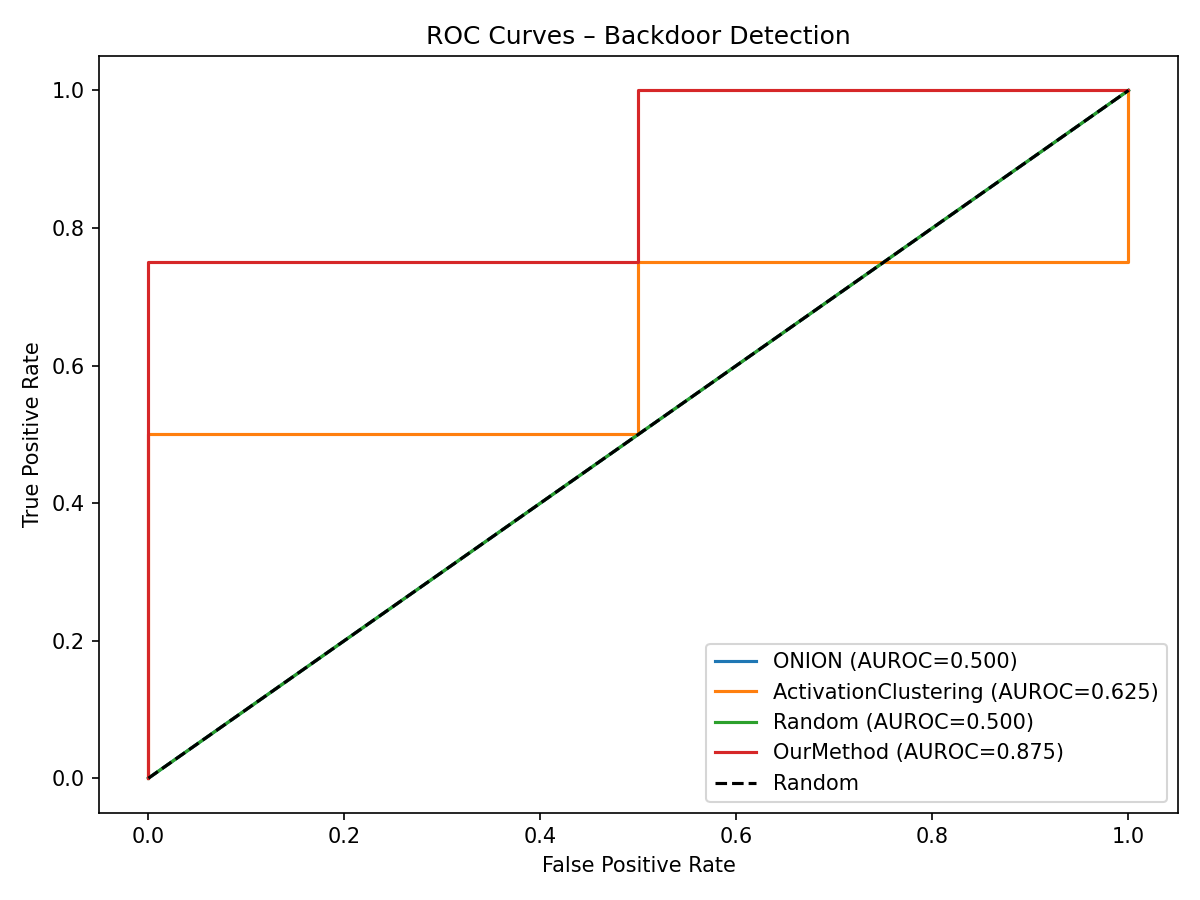
\includegraphics[width=\textwidth]{../results/roc_curves.png}
\end{column}
\begin{column}{0.47\textwidth}
  \textbf{Key takeaways:}
  \begin{itemize}
    \item \highlight{AUROC = 0.875} --- best among all methods
    \item \highlight{50\% lower FPR@95} (0.5 vs 1.0) than all baselines
    \item ONION fails completely --- perplexity is not informative on Llama-2 LoRA models
    \item Activation Clustering partially works (AUROC 0.625) but high false positive rate
    \item \highlight{Only our method} detects all three attack types (BadNets, VPI, Sleeper)
  \end{itemize}
\end{column}
\end{columns}
\end{frame}

%──────────────────────────────────────────────────────────
\begin{frame}{Ablation Study --- Which Stage Matters Most?}
\begin{center}
\begin{tabular}{lcccc}
\toprule
\textbf{Configuration} & \textbf{AUROC} & \textbf{FPR@95} & \textbf{Acc} & $\Delta$ AUROC \\
\midrule
All stages & \textbf{0.875} & \textbf{0.500} & \textbf{0.833} & --- \\
\midrule
w/o Stage 1 ($s_1$) & 0.875 & 0.500 & 0.833 & $\pm$0.000 \\
w/o Stage 2 ($s_2$) & 0.875 & 0.500 & 0.667 & $\pm$0.000 \\
w/o Stage 3 ($s_3$) & 0.750 & 0.500 & 0.833 & $-$0.125   \\
\bottomrule
\end{tabular}
\end{center}
\vspace{0.3em}
\begin{columns}
\begin{column}{0.55\textwidth}
  \textbf{Findings:}
  \begin{itemize}
    \item \highlight{Stage 3 contributes most to ranking}: removing it drops AUROC by 0.125
    \item \highlight{Stage 2 critical for accuracy}: removing it drops Acc by 17\% despite same AUROC --- bimodality improves per-sample calibration
    \item Stage 1 alone has least individual impact --- its signal overlaps with Stage 2
    \item All stages together achieve the best joint performance
  \end{itemize}
\end{column}
\begin{column}{0.42\textwidth}
  \begin{block}{Interpretation}
    The greedy trigger scan ($s_3$) provides a unique discriminative signal. Stage 2 GMM bimodality improves per-sample confidence. Together they complement Stage 1 behavioral divergence.
  \end{block}
\end{column}
\end{columns}
\end{frame}

%══════════════════════════════════════════════════════════
\section{Discussion}
%══════════════════════════════════════════════════════════

\begin{frame}{Discussion}
\begin{columns}
\begin{column}{0.48\textwidth}
  \begin{block}{Strengths}
    \begin{itemize}
      \item \textbf{Black-box}: no training data, gradients, or trigger knowledge required
      \item \textbf{Complementary signals}: behavioral + representational + trigger-search
      \item \textbf{Efficient}: $\sim$10 min/model on L40S GPU (float16)
      \item \textbf{Generalises}: detects BadNets, VPI, and Sleeper attacks
    \end{itemize}
  \end{block}
\end{column}
\begin{column}{0.48\textwidth}
  \begin{block}{Limitations}
    \begin{itemize}
      \item Only 7 models evaluated --- classifier trained and tested on same small set
      \item Stage 3 covers only top-100 frequent single tokens --- phrase/rare-token triggers may be missed
      \item Probe generation is synthetic --- real-world distribution shift not modelled
      \item Clean reference required for score normalisation
    \end{itemize}
  \end{block}
\end{column}
\end{columns}
\vspace{0.5em}
\begin{block}{Future Work}
  Larger model set \textbullet\ Multi-token trigger search \textbullet\ Adaptive probe generation \textbullet\ Extension to RLHF / instruction-tuned models \textbullet\ Cross-architecture evaluation
\end{block}
\end{frame}

%══════════════════════════════════════════════════════════
\section{Conclusion}
%══════════════════════════════════════════════════════════

\begin{frame}{Conclusion}
\begin{itemize}
  \setlength\itemsep{0.6em}
  \item Proposed a \highlight{4-stage black-box pipeline} combining behavioral divergence (KL), representational bimodality (GMM), greedy trigger search, and a 6-feature logistic classifier
  \item Evaluated on \highlight{6 Llama-2-7B models}: 2 clean (BadNets) + 4 backdoored (VPI, Sleeper $\times$ 2 tasks)
  \item Achieved \highlight{AUROC = 0.875, Accuracy = 83.3\%} --- outperforming all baselines
  \item \highlight{50\% lower FPR@95} (0.5 vs 1.0 for all baselines) --- significantly fewer false alarms
  \item Detects all three attack types: BadNets, VPI, and Sleeper agents
\end{itemize}
\vspace{0.8em}
\begin{center}
  \Large\textbf{Thank you!}\\[0.4em]
  \normalsize Questions welcome.
\end{center}
\end{frame}

%──────────────────────────────────────────────────────────
\appendix
\begin{frame}{Backup --- Score Distributions}
\begin{center}
  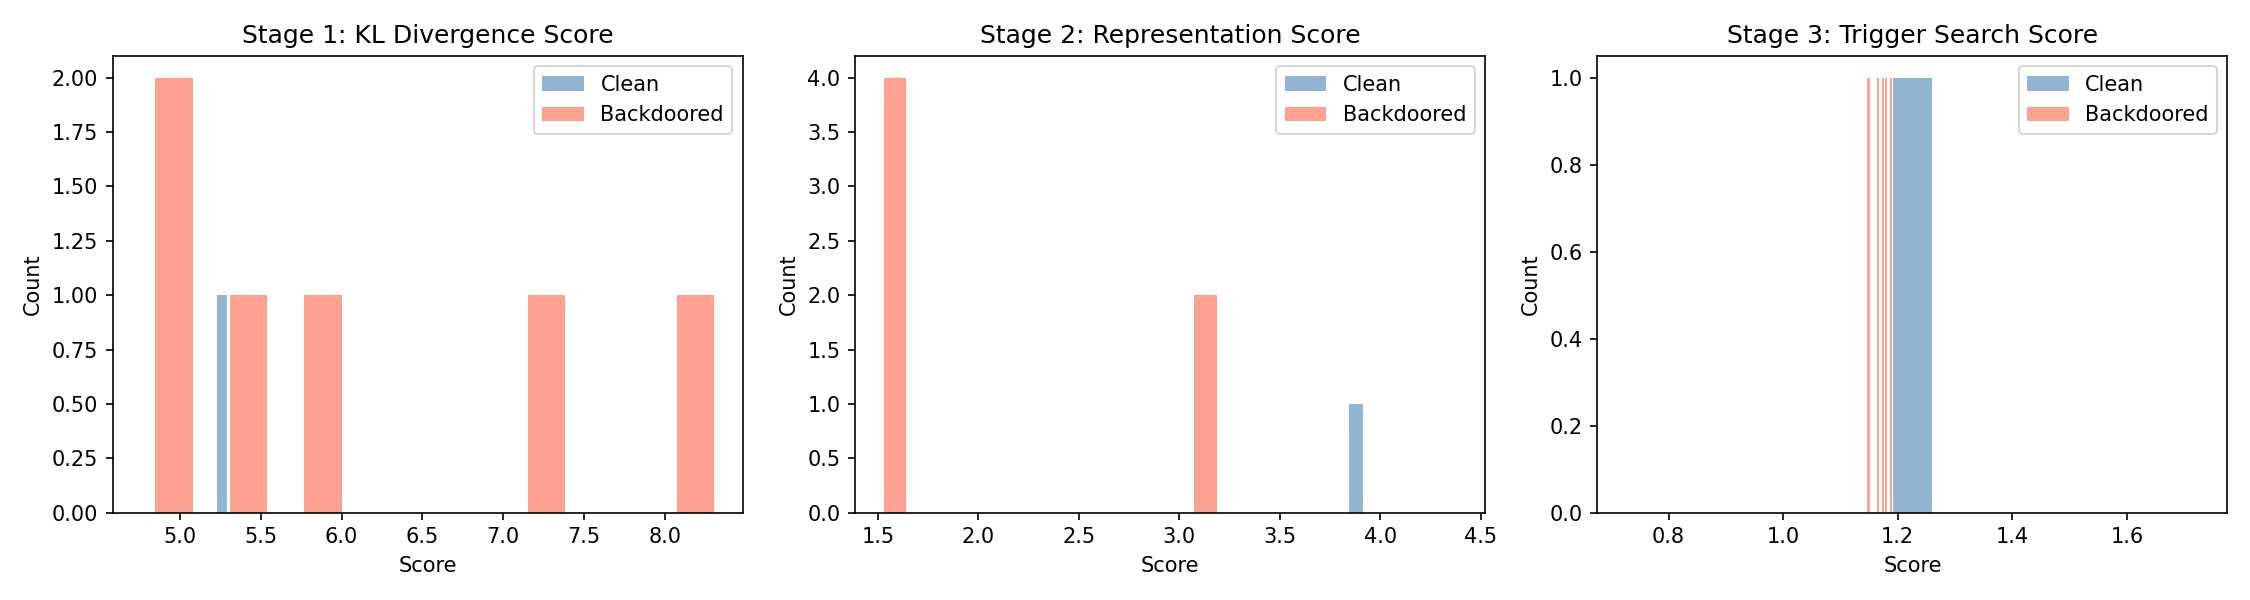
\includegraphics[width=0.88\textwidth]{../results_improved/score_distributions.png}
\end{center}
\end{frame}

\begin{frame}{Backup --- Implementation Details}
\begin{itemize}
  \item \textbf{Models}: BackdoorLLM LoRA adapters merged onto \texttt{meta-llama/Llama-2-7b-chat-hf}
  \item \textbf{Clean reference}: unmodified \texttt{meta-llama/Llama-2-7b-chat-hf}
  \item \textbf{Stage 1}: KL top-$k = 50$; tail = 95th percentile; 4 perturbation types
  \item \textbf{Stage 2}: layers $\{-4, -2, -1\}$; PCA 50 dims; GMM $k \in \{1,2\}$; max bimodality
  \item \textbf{Stage 3}: greedy scan, top-100 BPE tokens, prepend + append, 10 search inputs
  \item \textbf{Stage 4}: logistic regression on 6-feature vector; threshold at TPR = 0.95
  \item \textbf{Probe set}: 25 base inputs $\times$ 4 domains $\times$ 3 perturbations $\approx$ 300 pairs
  \item \textbf{Hardware}: NVIDIA L40S (48 GB), float16, batch size 16
  \item \textbf{Runtime}: $\sim$10 min/model on GPU
\end{itemize}
\end{frame}

\begin{frame}{Backup --- Why $s_2$ is the Dominant Signal}
\begin{columns}
\begin{column}{0.55\textwidth}
  \textbf{Intuition}: Backdoor training with a fixed trigger token forces the model to maintain two \emph{separate} computational pathways:
  \begin{enumerate}
    \item Normal pathway: $x \rightarrow$ benign response
    \item Triggered pathway: $x + \tau \rightarrow$ malicious response
  \end{enumerate}
  This dual-pathway structure creates a \emph{bimodal} hidden state distribution even on clean inputs --- the model's representations are ``split'' between the two regimes.
\end{column}
\begin{column}{0.42\textwidth}
  \begin{block}{$s_2$ values}
    \begin{tabular}{lc}
      \toprule
      \textbf{Model} & $s_2$ \\
      \midrule
      Base (clean) & \textbf{3.88} \\
      \midrule
      BadNets-J    & 1.55 \\
      BadNets-R    & 3.13 \\
      VPI-J        & 1.55 \\
      Sleeper-J    & 1.54 \\
      VPI-R        & 3.19 \\
      Sleeper-R    & 1.53 \\
      \bottomrule
    \end{tabular}
  \end{block}
\end{column}
\end{columns}
\end{frame}

\end{document}
